\section{Stochastic inference of surface-induced effects using Brownian motion}

\subsection{Confined Brownian motion theory}

By observing the trajectory along the $z$ axis of a particle of $1.5 ~ \mathrm{\mu m} $ as shown on the fig.\ref{Fig:exp_z_traj}, one can see that the particle height does not get heigher than $ \simeq 4 ~ \mathrm{\mu m}$. Indeed due to gravity, the particle is confined near the surface. Brownian motion in confinement and at interfaces is a canonical situation, encountered from fundamental biophysics  to  nanoscale  engineering. This confinement induces near-wall effects, such as hindered mobility and electrostatic interactions. 

In the first part of this chapter, I will detail the theory background of the confined Brownian motion and how to numerically simulate it. In a second part, I will present how to analyse experimental data. In particular, I will detail a multi-fitting procedure that allows a thermal-noise-limited inference of diffsion coefficients spatially resolved at the nanoscale, equilibrium potentials, and forces at the femtomewton resolution.

\begin{figure}[ht]
	\centering
	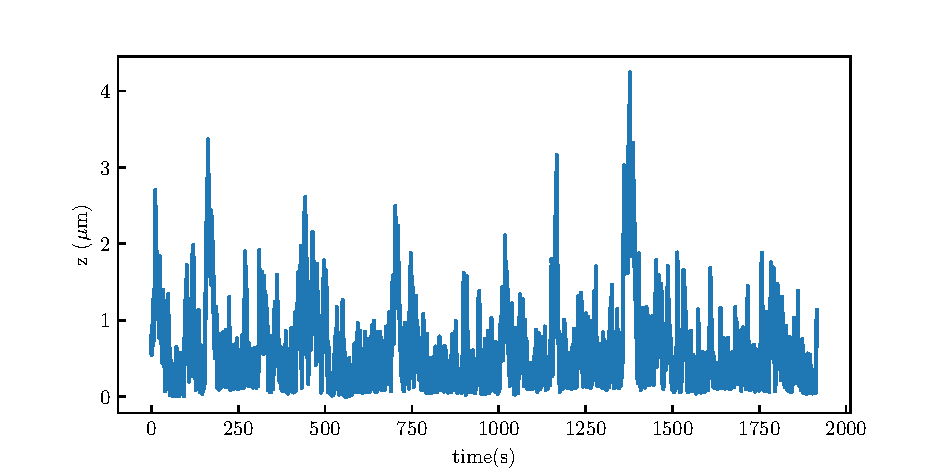
\includegraphics{02_body/chapter3/images/traj_z/traj_z.pdf}
	\caption{Experimental trajectory of a particule of polystyrene of radius $a = 1.5 ~ \mathrm{\mu m}$ near a wall ($z = 0$) along the $z$ axis --- perpendicular to the wall.}
	\label{Fig:exp_z_traj}
\end{figure}

\subsubsection{Gravitational interactions}

In our experiment, we observe confined Brownian motion since the colloids are subject to gravity. Indeed, the density of the observed colloid $\rho_\mathrm{p}$ is different of the medium $\rho_\mathrm{m}$ --- in our experiment water, $\rho_\mathrm{m} = 1000 ~ \mathrm{kg.m^{-3}}$. Thus, the particle lies into a gravitational potential given by:

\begin{equation}
	U_\mathrm{g} (z) = \Delta m g z = \frac{4}{3}\pi a ^3 g \Delta \rho z ~,
	\label{eq:ug_full}
\end{equation}

where $\Delta m$ is the mass difference of the particle and a fluid sphere of the same size, $\Delta \rho$ the corresponding density difference such as $\Delta \rho = \rho_\mathrm{m} - \rho_\mathrm{p} $ and $g$ the gravitational acceleration. By invoking the definition of a distance that we call the Boltzmann length,

\begin{equation}
	\ell _\mathrm{B} = \frac{k_\mathrm{B}T}{4/3 \pi a ^3 \Delta \rho g } ~,
\end{equation}

one can rewrite the gravitational potential Eq.\ref{eq:ug_full} as:

\begin{equation}
	U_\mathrm{g} = \frac{k_\mathrm{B}T}{\ell _\mathrm{B}} ~.
	\label{eq:ug}
\end{equation}

The Boltzmann length $\ell_\mathrm{B}$ is the typycal gravitational decay length and represents the balance between the gravital potential and thermal energy. This distance was first measured by Perrin \cite{perrin_les_2014}, by enumerating the number of particles as a function of height to reconstruct the concentraction of the colloidal suspension that exponentially decays as $e^{- z / \ell _\mathrm{B}}$. As an exemple, in water, for a particle polystyrene, $\rho _\mathrm{p} = 1050 ~ \mathrm{kg.m^{-3}}$ and of radius $a  = 1.5 ~ \mathrm{\mu m}$ we have $\ell _\mathrm{B} = 0.58 ~ \mathrm{\mu m}$.

For particle with $\ell _\mathrm{B} >> a $, one can consider that the particle does not feel the gravity. This is particulary the case when the density of the colloids and fluid matches, in this particular case $\ell _\mathrm{B} = 0$. Thus density matching can we a way to do grativation free experiments. In the case of our experiment, we want to measure confinement induced effects, therefore, we need this gravitational interaction to have the particles near the surface. Indeed, as a particle gets larger, or, denser $\ell _\mathrm{B}$ decreases and the particle will be, in average, closer to the surface. 


\subsubsection{Doube-layer electrostatic interactions}

When a surface in immerge in water are usually charged \cite{israelachvili_intermolecular_2015} due to an high dieletric constant $\epsilon \simeq 80$ that permit the build up of charges for low energetic price. Commonly, surface charging is done through ionization of dissociation of surface groups\footnote{For example, the dissociation of protons from surface carboxylic groups \cite{israelachvili_intermolecular_2015} ($-$COOH $\rightarrow$ -COO$^-$ + H$^+$) which charge negatively the surface.}, from the binding of ions from the solution --- for example, adsorption of $-$OH$^-$ onto the the water-air interface that charge it negatively. In the bulk, a fluid should be electrically neutral, thus the fluid contains as many ions of opposite charge. However, when a surface is charged negatively, negative ions are repelled from the surface, while positive ions are attracted towards the surface.  Therefore, a double-layer charge distribution is formed near the surface, as shown Fig.XX. Experimentally, we use glass slides and polystyrene beads, that are both negatively charged in water, thus leading to repulsive double-layer. This repulsive force prevent the colloids to stick together or to the surface of the substrat. 






\begin{figure}[h]
	\centering
	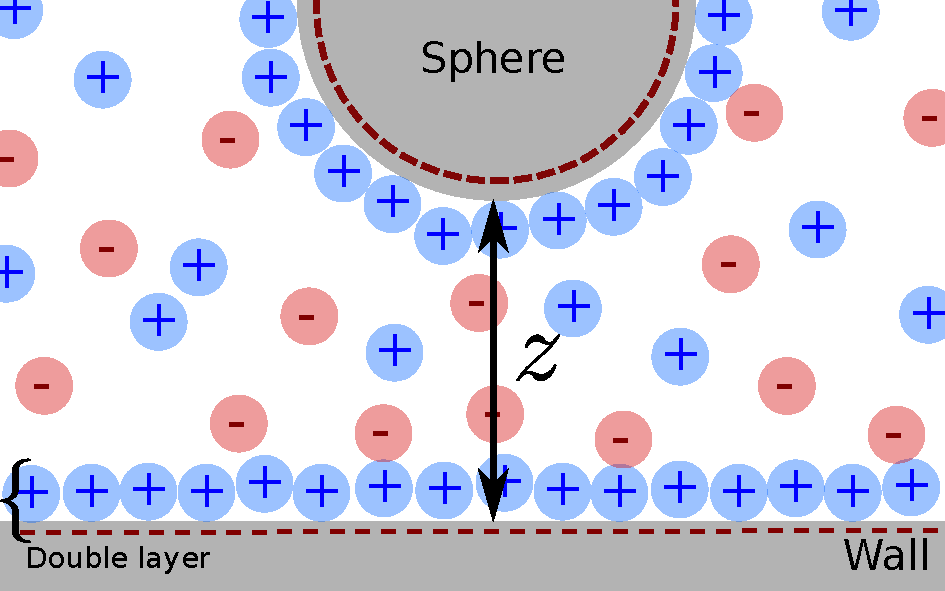
\includegraphics{02_body/chapter3/images/double_layer.pdf}
	\caption{A Brownian colloid diffusing near a wall. Both wall and colloid's surface charge negatively, in consequence, a layer of positively charge ions are towards the surfaces, forming a double-layer charge distribution.}
	\label{Fig:double_layer}
\end{figure}




If the solution contains an electrolyte, for example a salty solution, containing Na$^+$ and Cl$^-$ ions. The electrostatic potential $\Psi(\vec{r})$ generated by the double layer satifies Poisson's equation \cite{israelachvili_intermolecular_2015}:

\begin{equation}
	\nabla ^2 \Psi(\vec{r}) = -\frac{1}{\epsilon_r \epsilon_0}  \rho_e(\vec{r})~,
	\label{Eq:poisson}
\end{equation}

where $\epsilon_0$ the vacuum permittivity, $\epsilon_r$ the relative permitivity of the fluid, $\rho_e(\vec{r})$ the local charge density. The latter can be written as:

\begin{equation}
	\rho_e(\vec{r}) = e \sum _i z_i c_i (\vec{r}) ~,
	\label{Eq.3}
\end{equation}

where $e$ is the elementary charge, $i$ denotes an ionic species of valence $z_i$ and local concentration $c_i(\vec{r})$. If the solution is at the thermodynamic equilibrium, the Boltzmann equation is used to calculate the local ion density such that:

\begin{equation}
	c_i(\vec{r}) = c_i ^0 \textnormal{exp}\left(\frac{z_i e \Psi(\vec{r})}{k_\mathrm{B} T }\right) ~,
	\label{Eq.4}
\end{equation}


where $c_i ^0$ is the bulk concentration of the ionic species $i$. By combining Eqs.\ref{Eq:poisson}, \ref{Eq.3} and \ref{Eq.4}, one can obtain the Poisson-Boltzmann equation:

\begin{equation}
	\nabla ^2 \Psi (\vec{r}) = \sum_i \frac{z_i e c_i^0}{\epsilon_0 \epsilon_r} \exp \left( - \frac{z_i e \Psi (\vec{r})}{k_\mathrm{B}T} \right) ~.
	\label{Eq:Poisson-boltzmann}
\end{equation}

Since the Poisson-Boltzmann is non-linear, it is most likely to be solve numerically. However, for simple geometry such as uniformly charged plane or sphere it can be solve analiticaly. Let consider, to simplify, that we have a monovalent electrolyte, meaning that the electrolyte is composed of two ions of valence equal to one --- Na$^+$ Cl$^-$ for example --- and $c_i ^0$ is equal to the electrolyte solution concentration $c_s^0$. In that case Eq.\ref{Eq:Poisson-boltzmann} simplifies to:

\begin{equation}
	\begin{aligned}
	\nabla ^2 \Psi (\vec{r}) &= \frac{e c_s ^0}{\epsilon_0 \epsilon_r} \left[ \exp \left( \frac{-e\Psi(\vec{r})}{k_\mathrm{B}T} \right) -  \exp \left( \frac{+e\Psi(\vec{r})}{k_\mathrm{B}T} \right) \right] \\
	& = 2 \frac{e c_s ^0}{\epsilon_0 \epsilon_r} \mathrm{sinh}  \left( \frac{e\Psi(\vec{r})}{k_\mathrm{B}T} \right) ~.
	\end{aligned}
\end{equation}

In the case, where the $\Psi$ is small enough everywhere to have the electrostatic potential energy $e\Psi << k_\mathrm{B} T$, which generally the case when using salty solution. In that case, it is possible, using the a Taylor approximation at the second order to write:

\begin{equation}
	\exp \left( - \frac{z_i e \Psi(\vec{r})}{k_\mathrm{B}T} \right) \simeq 1 + \frac{z_i e \Psi (\vec{r})}{k_\mathrm{B}T} ~.
\end{equation}

Thus, the Poisson-Boltzmann equation (Eq.\ref{Eq:Poisson-boltzmann}) becomes:

\begin{equation}
	\nabla ^2 \Psi (\vec{r}) = \sum_i \frac{z_i e c_i^0}{\epsilon_0 \epsilon_r}  \left( 1 + \frac{z_i e \Psi (\vec{r})}{k_\mathrm{B}T} \right) ~.
\end{equation}

Since the fluid in the bulk, is electrically neutral, the first term vanishes as $\sum_i z_i c_i^0 = 0$. One thus have a linearized version of Eq.\ref{Eq:Poisson-boltzmann}, which is known as the Debye-Hünkel equation:

\begin{equation}
	\nabla^2 \Psi (\vec{r}) = \left[  \sum_i \frac{z_i ^2 e^2 c_i^0}{\epsilon_0 \epsilon_r  k_\mathrm{B} T}    \right] \Psi (\vec{r}) ~.
\end{equation}

From this approximation, one can identify that the term between brackets is the inverse of a distance squared. We can thus define a distance $\ell _\mathrm{D}$, the Debye length such as:

\begin{equation}
	\ell _\mathrm{D} =  \sqrt{ \sum_i\frac {\epsilon_0 \epsilon_r k_\mathrm{B} T} {z_i ^2 e^2 c_i^0}} ~.
\end{equation}

The Debye length...






\subsubsection{Local diffusion coefficient}



We have seen that the bulk Brownian motion is well known and documented for a long time. But, in the real world, the boundaries are not at infinity and could play a role in the process of diffusion. Indeed, it was theorized by H. Faxen \cite{faxen_fredholm_1924} that the presence of a wall would change the Stokes-Einstein relation with a viscosity dependent to the position of the particle. As the particle get closer to a surface, the presence of the non-slip boundary condition make the fluid harder to push, thus increasing the local viscosity of the particle. This variation of the viscosity will be different for orthogonal and parallel displacement to the wall, thus we write respectively $\eta_\bot $ and $\eta_\parallel$ with $\eta_0$ being the fluid viscosity and $z$ the height of the particle:

\begin{equation}
	\eta_\bot = \frac{4}{3} \eta_0 \mathrm{sinh}\beta \sum _{n=1} ^{\infty} \frac{n(n+1)}{{2n-1}{2n+3}}
	\left[
	\frac
	{
		2\mathrm{sinh}(2n + 1)\beta + (2n +1)\mathrm{sinh}2\beta
	}
	{
		4\mathrm{sinh}^2(n + 1 /2)\beta  - (2n+1)^2 \mathrm{sinh}^2 \beta
	}
	-1
	\right] ~,
	\label{Eq:etaz}
\end{equation}

\nomenclature{$\eta_\bot$}{Viscosity orthogonal to a wall, see Eq.\ref{Eq:etaz}}
and 

\begin{equation}
	\eta_\parallel = \eta_0 
	\left[
	1 - \frac{9}{16} \xi + \frac{1}{8}\xi^3 - \frac{45}{256}\xi^4 - \frac{1}{16}\xi^5
	\right]^{-1}~,
	\label{Eq:etax}
\end{equation}
\nomenclature{$\eta_\parallel$}{Viscosity parrallel to a wall, see Eq.\ref{Eq:etax}}

where $\xi = \frac{a}{z+a}$ and $\beta = \mathrm{cosh}^{-1}(\xi)$. It is possible to simplify the form of $\eta_\bot$ by using a Padé approximation, which is correct up to $1\%$ of accuracy:

\begin{equation}
	\eta_\bot = \eta_0 \frac{6z^2 + 9az + 2a^2}{6z^2 + 2az}~.
\end{equation}

Of course, this local viscosity is directly reflected on the diffusive properties of the particle, hence a local diffusion coefficient, which we write:

\begin{equation}
	D_i (z) = \frac{k_\mathrm{B} T}{6\pi\eta_i (z) a}~.
\end{equation}

One of the first experimental measurement of the local diffusion coefficient was brought by Faucheux and Libchaber \cite{faucheux_confined_1994} where they measured the mean diffusion coefficient with various gaps and particle radius their results can be found in the Fig.\ref{fig:libchaber}.

\begin{figure}
	\centering
	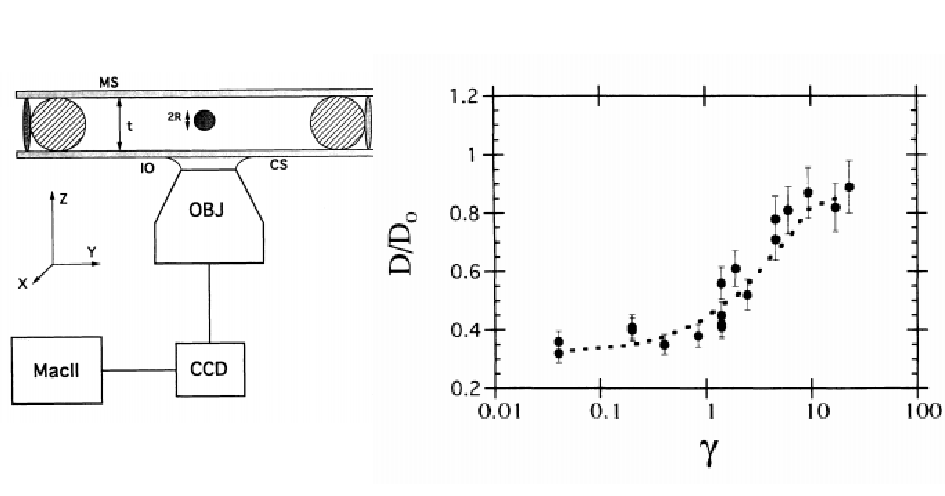
\includegraphics{02_body/chapter1/image/libchaber.pdf}
	\caption{Figure extracted from \cite{faucheux_confined_1994}, on the left is the experimental setup used. It is an inverted microscope used in order to track particle of size $2R$ inside a cell of thickness $t$. On the right is their final result, where they measure the diffusion parallel coefficient $D_\bot$ given by Eq.\ref{Eq:etax}, here normalized by $D_0$ the bulk diffusion coefficient as a function of  $\gamma$ a confinement constant $\gamma = (\langle z \rangle -a)/a$. }
	\label{fig:libchaber}
\end{figure}

Another interesting physical aspect to take into account when looking at confined Brownian motion is the potential the particle is lying into. Let's first consider the weight of the particle. Indeed, if the particle density does not match the fluid' one, a spherical particle will lye in a gravity potential given by:

\begin{equation}
	U_g(z) = \frac{4}{3} \pi a^3 (\rho_\mathrm{P} - \rho_\mathrm{F})gz~,
\end{equation}

\nomenclature{$g$}{Gravity constant}
\nomenclature{$\rho_\mathrm{P}$}{Particle density}
\nomenclature{$\rho_\mathrm{F}$}{Fluid density}

that we can rewrite for simplicity

\begin{equation}
	\frac{U_g(z)}{k_\mathrm{B} T} = \frac{z}{\ell_\mathrm{B}}~,
\end{equation}

\nomenclature{$\ell_\mathrm{B}$}{Boltzmann length}
with $\ell_\mathrm{B}$ the Boltzmann length which represents the balance between the kinetic energy and the weight of the particle:

\begin{equation}
	\ell_\mathrm{B} = \frac{k_\mathrm{B} T}{ \frac{4}{3} \pi a^3 \Delta \rho g}~.
\end{equation}

Let's now consider the interactions with the substrate, glass slides when immersed in water do charge negatively as well as polystyrene particles that we use. We will then have repulsive electrostatic interactions between the wall and the particles, the corresponding potential can be written as  \cite{israelachvili_intermolecular_2015}:

\begin{equation}
	\frac{U_\mathrm{elec}(z)}{k_\mathrm{B}T} = B \mathrm{e}^{-z/\ell_\mathrm{D}}~,
\end{equation}

\nomenclature{$B$}{Amplitude of the electrostatic interactions}
\nomenclature{$\ell_\mathrm{D}$}{Debye length}

where $B$ is the amplitude of electrostatic interactions, representing the surface charges and $\ell_\mathrm{D}$ being the Debye length, which is the characteristic length of the electrostatic interactions. The particle is thus lying in a total potential given by:

\begin{equation}
	\frac{U(z)}{k_\mathrm{B}T} =   B \mathrm{e}^{-z/\ell_\mathrm{D}} +  \frac{z}{\ell_\mathrm{B}}~.
\end{equation}

From this total potential one can construct the Gibbs-Boltzmann distribution in position:

\begin{equation}
	P_\mathrm{eq}(z) = A\mathrm{e}^
	{
		\frac{U}{k_\mathrm{B}T}	
	}~,
	\label{Eq:Peq}
\end{equation}

where $A$ is a normalization constant so that $\int P_\mathrm{eq} = 1$. This distribution gives us the probability to find the particle at a height $z$. The exponential decay due to the gravity was first measured by Perrin \cite{perrin_les_2014} by methodically counting through a microscope the number of colloids in suspension as a function on the height. 


\begin{figure}[ht]
	\centering
	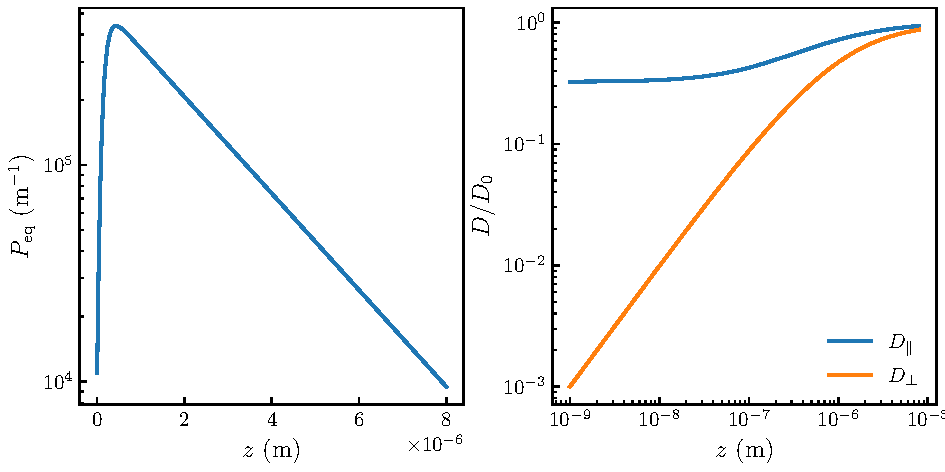
\includegraphics{02_body/chapter1/image/theorie_chap1.pdf}
	\caption{On the left, plot of the Gibbs-Boltzmann distribution Eq.\ref{Eq:Peq} for $a = 1 ~ \mathrm{\mu m}$, $ B = 4 $, $\ell _\mathrm{D} = 100 ~ \mathrm{nm}$ and $\Delta \rho = 50 ~ \mathrm{kg.m^{-3}}$. On the right, local diffusion coefficient normalized by bulk diffusion coefficient $D_0 = k_\mathrm{B}T/\gamma$, given by Eq.\ref{Eq:etax} and Eq.\ref{Eq:etaz}}.
\end{figure}








\subsubsection{Langevin equation for the Brownian motion}



\subsubsection{Spurious drift}

\subsubsection{Numerical simulation of confined Brownian motion}

\subsection{Experimental study}

\subsubsection{MSD}

\subsubsection{Non-gaussian dynamics - Displacement distribution}

\subsubsection{Local diffusion coefficient inference}

\subsubsection{Precise potential inference using multi-fitting technique}

\subsubsection{Measuring external forces using the local drifts}

\subsection{conclusion}
